\documentclass[14pt]{extarticle}
\usepackage[]{cite}
\usepackage{cmap}
\usepackage[T2A]{fontenc}
\usepackage[utf8]{inputenc}
\usepackage[english, russian]{babel}
\usepackage{amsmath, amsfonts,amssymb,mathrsfs}
\usepackage{graphicx, epsfig}
\usepackage{subfig}
% \usepackage{color}
\usepackage{algorithm}
\usepackage{algorithmic}
\floatname{algorithm}{Алгоритм}
\usepackage{hyperref}
\usepackage{mathrsfs}

\usepackage{wrapfig}
\usepackage{float}
\usepackage{subfloat}
\usepackage{caption}
\usepackage{multirow}
\usepackage{dsfont}
\graphicspath{{./img/}}
% \usepackage{xcolor}
% \usepackage[dvipsnames]{color}
\usepackage[dvipsnames]{xcolor}
\definecolor{mynicegreen}{RGB}{102,252,102}

\newcommand\argmin{\mathop{\arg\min}}
\DeclareMathOperator*{\argmax}{argmax}
\newcommand{\T}{^{\text{\tiny\sffamily\upshape\mdseries T}}}
\newcommand{\hchi}{\hat{\boldsymbol{\chi}}}
\newcommand{\hphi}{\hat{\boldsymbol{\varphi}}}
\newcommand{\bchi}{\boldsymbol{\chi}}
\newcommand{\A}{\mathcal{A}}
\newcommand{\B}{\mathcal{B}}
\newcommand{\x}{\mathbf{x}}
\newcommand{\hx}{\hat{x}}
\newcommand{\hy}{\hat{y}}
\newcommand{\M}{\mathcal{M}}
\newcommand{\N}{\mathcal{N}}
\newcommand{\R}{\mathbb{R}}
\newcommand{\p}{p(\cdot)}
\newcommand{\q}{q(\cdot)}
\newcommand{\uu}{\mathbf{u}}
\newcommand{\vv}{\mathbf{v}}


\renewcommand{\baselinestretch}{1}


\newtheorem{Th}{Теорема}
\newtheorem{Def}{Определение}
\newenvironment{Proof} % имя окружения
    {\par\noindent{\bf Доказательство.}} % команды для \begin
    {\hfill$\scriptstyle\blacksquare$} % команды для \end
\newtheorem{Assumption}{Предположение}
\newtheorem{Corollary}{Следствие}

\textheight=22cm % высота текста
\textwidth=16cm % ширина текста
\oddsidemargin=0pt % отступ от левого края
\topmargin=-1.5cm % отступ от верхнего края
\parindent=24pt % абзацный отступ
\parskip=5pt % интервал между абзацами
\tolerance=2000 % терпимость к "жидким" строкам
\flushbottom % выравнивание высоты страниц



\begin{document}

\thispagestyle{empty}
\begin{center}
    \sc
        ФГАОУВО «Московский физико-технический институт \rm{(национальный исследовательский университет)}»\\
        Физтех-школа аэрокосмических технологий\\
        Кафедра компьютерного моделирования\\[20mm]
    \begin{flushleft}
  \textbf{Направление подготовки:} 01.03.02 Прикладные математика и информатика (бакалавриат) \\
  \textbf{Направленность (профиль) подготовки:} Прикладные математика и информатика \\
  \textbf{Форма обучения:} очная\\[20mm]
  
    \end{flushleft}
    
    \bf\
		ВЫПУСКНАЯ КВАЛИФИКАЦИОННАЯ РАБОТА \\ «Прогнозирование деградации турбовентиляторных реактивных двигателей с помощью методов глубинного обучения»\\

    
\end{center}
	
	\begin{center}
		(бакалаврская работа)\\[15mm]
  	\end{center}
	
		

\hfill\parbox{80mm}{
    \begin{flushleft}
    \bf
        Студент:\\
    \rm
        Теслюк Никита Александрович \\[1cm]
    \bf
        Научный руководитель:\\
    \rm
        к.~ф.-м.~н. \\ Аврутский Всеволод Игоревич \\[2cm]
    \end{flushleft}
}
\begin{center}
    Жуковский\\
    2021
\end{center}


\newpage
\tableofcontents
\newpage




\section{Введение}
\label{sec:intro}

Многие авиакомпании в последние годы уже получили выгоду от использования искусственного интеллекта (AI --- {\it artificial intelligence}) для мониторинга состояния двигателя (EHM --- {\it engine health monitoring}) и приступили к кампаниям по оптимизации программ, призванным сдерживать расходы и повышать надежность летательных судов. Но, стоит отметить, что относительно немногие преуспели в первых попытках применить ИИ к гораздо более сложным средам обслуживания компонентов и линий, такие как двигатели. Прогностическая сила ИИ может способствовать резкому увеличению прибыльности авиакомпаний за счет устранения сбоев в работе, вызванных техническим обслуживанием, а также повышению безопасности пассажиров.

Анализируя массив исторических данных по техническому обслуживанию воздушных судов и показаний датчиков двигателей, система позволяет прогнозировать в долгосрочной перспективе возможные дефекты по каждому отдельно взятому самолёту. Система способна определять вероятность возникновения разных типов дефектов в определенный период в будущем. В случае, если вероятность оказывается выше установленного порога, рекомендуется провести дополнительную проверку воздушного судна.

Исходя из того, что данные, снятые с датчиков, установленных в разных частях двигателя, в большинстве своём являются временными рядами, возникает идея применения современных нейросетевых state-of-the-art подходов глубинного обучения, используемых для работы с последовательностями, таких как рекуррентные нейронные сети и их модификации (RNN, LSTM). Также в долгосрочной перспективе для повышения точности предсказания возможно использование Attention-based подходов из области NLP ({\it natural language processing}), предлагаемых в архитектуре Transformer.

В данной работе рассматривается применение модели LSTM ({\it Long Short Term Memory}). Главным преимуществом LSTM моделей над классическими RNN является то, что они способны "запоминать" долгосрочные зависимости. Эти модели очень хорошо работают с большим спектром задач и в настоящее время широко используются.

Таким образом, {\bf основной целью} данной работы является разработка прогнозирующей модели на основе LSTM, а также сравнение ее точности с классическими алгоритмами машинного обучения для решения задач регрессии и прогнозирования, таких как случайный лес, градиентный бустинг и др. 

С точки зрения практического исполнения данная работа включает в себя имплементацию модели LSTM. Код, воспроизводящий эксперименты, размещен по ссылке \href{https://github.com}{https://github.com}

\newpage

\section{Обзор литературы}

\newpage

\section{Задача прогнозирования}

\subsection{Постановка задачи}

Заданы:
\begin{itemize}

    \item $U = \left\{ u_j|\ u_j \in \mathbb{R}^k,\ j \in 1,\dots n_{users} \right\}$ --- множество субъектов (пользователей/users), для удобства преобразованных в векторы. Это преобразование можно сделать например с помощью матричной факторизации или VAE \cite{vae}.
    \item $I = \left\{ i_j|\ i_j \in \mathbb{R}^k,\ j \in 1,\dots n_{items} \right\}$ --- множество объектов (рекомендуемых фильмов/items), преобразованных в векторы той же размерности, что и пользователи.
    \item $R = \| r_{ui}\|$ --- матрица рейтингов размера $n_{users}\times n_{items}$, $r_{ui}\in \overline{1, 5}$

\end{itemize}

В рекомендательных системах существуют различные постановки задач, такие как прогнозирование неизвестных рейтингов $r_{ui}$, оценивание сходства $\rho (u, u'),\ \rho (i, i'),\ \rho (u, i)$ и т.~д. В данной работе исследуются методы, формирующие список рекомендаций для пользователей.

Более формально, для каждого пользователя $u\in U$ требуется построить список $y = \left\{y_j\right\}_{j=1}^{N}$ из наиболее релевантных объектов, отсортированный по убыванию.

Для того, чтобы определять, насколько построенный алгоритмом список соответствует истинным значениям релевантности, введём два критерия качества:

$$HR@p(y)=\sum\limits_{j=1}^{p} rel_{y_j};$$

$$DCG@p(y)= \sum\limits _{{j=1}}^{{p}}{\frac  {rel_{y_j}}{\log _{{2}}(j+1)}};$$
где $rel_{y_j}=1$, если объект $y_j$ релевантен ($r>3$), иначе 0.

Первый критерий (Hit Rate) считает количество релевантных объектов среди первых $p$ элементов списка. Второй (Discounted Cumulative Gain) дополнительно дисконтирует это количество, учитывая позицию в рекомендованном списке. Поскольку важнее правильно выдавать наиболее релевантные объекты, для знаменателя больше подходит логарифм порядкового номера из списка, а не этот номер напрямую. 

В дальнейшем будем оптимизировать усреднённые значения этих критериев по всем подвыборкам (батчам) из тестовой выборки.

\subsection{Сведение к задаче обучения с подкреплением} 

Традиционные подходы к решению задачи рекомендаций используют коллаборативную фильтрацию \cite{CF_MF, GoogleNewsCF} или контентно-основанные рекомендации \cite{content-based, content-based_news}. Эти методы имеют ряд недостатков: проблема холодного старта, отсутствие возможности онлайн-обучения, необходимость хранить в памяти всю матрицу рейтингов. Кроме того, такие подходы основываются
на исторических данных и не учитывают постоянно возникающих новых интересов пользователей.

\begin{figure}[h]
	\centering
	\includegraphics[width=0.85\textwidth]{img/consecutive.png}
	\caption{Анализ последовательных рекомендаций. Взято из \cite{Liu2018DeepRL}}
	\label{fig:consequtive}
\end{figure}

В работе \cite{Liu2018DeepRL} (рис.~\ref{fig:consequtive}) показан пример того, как начальные рекомендации влияют на дальнейшие оценки пользователей. Видно, что если система последовательно рекомендует пользователю релевантные товары, то он будет склонен ставить более высокие оценки и наоборот. Это показывает, что рекомендации пользователю следует рассматривать как последовательный процесс принятия решений.

Стандартным подходом к решению подобных задач является обучение с подкреплением. Оно позволяет явно использовать последовательность действий пользователя, чтобы лучше подстраиваться под его интересы. 

\newpage

\section{Обучение с подкреплением}

\subsection{Постановка задачи}

В задачах обучения с подкреплением рассматривается агент, взаимодействующий со средой. Конечная цель --- научить агента совершать оптимальные действия для достижения заданной цели.

Задано множество $\mathcal{S}$ состояний среды и множество $\mathcal{A}$ доступных действий агента.
Введём также функцию переходов $\mathcal{P}: \mathcal{S} \times \mathcal{A} \times \mathcal{S} \rightarrow [0, 1]$.

Согласно гипотезе Р. Саттона, автора книги \cite{sutton_book}, произвольные цели и задачи могут быть сформулированы как максимизация математического ожидания суммы последовательно полученного скалярного сигнала. В обучении с подкреплением сигнал, получаемый от среды, называется функцией награды $\mathcal{R} :\ \mathcal{S} \times \mathcal{A} \times \mathcal{S} \rightarrow \mathbb{R}$.

В момент времени $t$ агент наблюдает состояние среды $s_t\in \mathcal{S}$, совершает действие $a_t\in \mathcal{A}$ в соответствии со свой стратегией (политикой, policy) $\pi:\ \mathcal{S} \times  \mathcal{A} \rightarrow [0, 1]= \mathbb{P}(a_t|s_t)$, переходит в состояние $s_{t+1}$ и получает награду $r_t$.

Часто удобно задавать стратегию агента в параметрическом виде:
$\pi_{\theta} = \mathbb{P} (a|s, \theta)$. 
Решить задачу обучения с подкреплением означает найти стратегию, максимизирующую дисконтированную сумму наград:

% \begin{equation}
$$J(\theta) = \mathbb{E}_{\pi_{\theta}} \left[ \sum\limits_{k=0}^{\infty} \gamma^k r_{t+k}\right] \rightarrow \max_{\pi_{\theta}},$$
% 	\label{expected_return}
% \end{equation}
где $\gamma \in [0, 1)$ --- параметр дисконтирования, гарантирующий, что бесконечная сумма не будет расходиться при конечных значениях награды. 

\subsection{Среда для рекомендательной системы}

\begin{enumerate}

\item

Вектор состояния среды будем описывать аналогично \cite{Liu2018DeepRL}. Он состоит из вектора текущего пользователя $u$, вектора, отражающего $n$ последних релевантных для него объектов и вектора, содержащего их попарные произведени (рис.~\ref{fig:state}).

\begin{figure}[h]
	\centering
	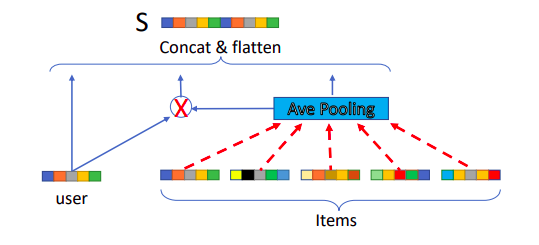
\includegraphics[width=0.6\textwidth]{img/state_representation.png}
	\caption{Описание состояния среды. Взято из \cite{Liu2018DeepRL}}
	\label{fig:state}
\end{figure}

$s = \left[u, u \otimes \{w_l i_l\ |\ l = 1, ..., n\}, \{w_l i_l\ |\ l = 1,\dots, n\}\right] \in \mathbb{R}^{3k} ,$

где $w_l$~---~веса понижающего размерность слоя, показывающие важность объекта $i_l$, а символом $\otimes$ обозначено поэлементное произведение.

\item
Действия агента удобно задавать с помощью вектора $a\in \mathbb{R}^k$, следуя статье \cite{wolpertinger}. Пользователю рекомендуется объект, скалярное произведение которого с вектором $a$ наибольшее:

$$i = \underset{i_j\in \mathcal{A}}{\argmax}\ i_j a^T,$$

\item

Наконец награды будем задавать следующим образом 

($r_t\in \mathcal{R}, r_{ui} \in R$):

$$r_t= 
\begin{cases}
    1,& \text{если}\ r_{ui} > 3\\
    0,              & \text{иначе}
\end{cases}
$$
\end{enumerate}

\subsection{Методы решения}

В обучении с подкреплением можно выделить 2 типа методов (см. рис.~\ref{fig:components}).

\begin{figure}[h]
	\centering
	\includegraphics[width=0.4\textwidth]{img/rl_prospect.pdf}
	\caption{Группы алгоритмов обучения с подкреплением}
	\label{fig:components}
\end{figure}

В первой группе (model-based) выучивается модель среды $p(s_{t+1}|s_t, a_t)$, что требует большого количества наблюдений и времени.
В ранних работах, например в \cite{mdp} предпринимались попытки использовать model-based подходы, однако это мало применимо для рекомендательных систем из-за высокой ресурсозатратности, далее этот подход рассматриваться не будет.

Алгоритмы из второй группы либо выучивают функцию ценности и используют её для формирования стратегии (value-based), либо параметризуют стратегию и обновляют её напрямую (policy-based), либо делают и то и то (actor-critic). В работе исследуется метод, относящийся к классу актор-критик. Для целостности изложения кратко опишем все три класса алгоритмов.

\subsubsection{Value-based}
Введём функцию ценности:
$$V^{\pi}(s) = \mathbb{E}_{\pi} \left[ \sum\limits_{k=0}^{\infty} \gamma^k r_{t+k+1} | s_t=s\right]$$
и Q-функцию:
$$Q^{\pi}(s, a) = \mathbb{E}_{\pi} \left[\sum\limits_{k=0}^{\infty} \gamma^k r_{t+k+1} | s_t=s, a_t=a \right]$$

Выучив оптимальное значение Q-функции можно задать стратегию, например как $\pi(s_t) = \argmax\limits_{a_t} Q(s_t, a_t)$

В непрерывных средах трудно применять напрямую данный подход, поскольку это требует жадной оптимизации на каждом шаге.
Вместо этого воспользуемся подходом актор-критик, где критик будет выучивать $Q$ - функцию, а актор --- политику. Для этого предварительно опишем часть, связанныю с актором в следующем подразделе.

\subsubsection{Policy-based}

Алгоритмы, основанные на оптимизации политики, обновляют параметры $\pi_{\theta}$, максимизируя ожидаемую награду $J(\theta)$.
$\nabla_{\theta} J(\theta)$ можно рассчитать, используя результат из \cite{pg} (считая $\pi_{\theta}$ дифференцируемой по $\theta$):

$$ \nabla_{\theta} J(\theta) = \mathbb{E}_{s\sim \rho^{\pi}, a\sim \pi_{\theta}} \ \left[\nabla_{\theta} \log \pi_{\theta} (a|s) Q^{\pi}(s, a)\right],$$

где дополнительно введено распределение состояний с учётом дисконтирования $\rho^{\pi}(s) = \sum\limits_{t=1}^{\infty} \gamma^{t-1} \mathbb{P} (s_t=s|s_0, \pi)$

Истинные значения $Q$ - функции обычно неизвестны, их можно заменить например на дисконтированные суммы полученных в сессии наград.

\subsubsection{Actor-Critic}

В подходе актор-критик обучается и параметризованная $Q$-функция $Q_{\theta^Q}(s, a)$ (критик) и политика $\pi_{\theta}$ (актор), так что для вычисления $\nabla_{\theta} J(\theta)$ используется значение $Q_{\theta^Q}(s, a)$.

Заметим, что вычисление $\nabla_{\theta} J(\theta)$ требует интегрирования и по пространству состояний, и по пространству действий, что требует большего количества данных, особенно при больших размерностях. Традиционным является подход с использованием детерминированной политики, для неё градиент ожидаемой награды $\nabla_{\theta} J(\theta)$ имеет вид \cite{dpg}:

$$ \nabla_{\theta} J(\theta) = \mathbb{E}_{s\sim \rho^{\pi}} \ \left[ \nabla_a Q(s, a)|_{a = \pi(s)}\nabla_{\theta^{\pi}} \pi (s)\right]$$

В результате получим следующий алгоритм:

\begin{algorithm}[H]
\caption{{Deep Deterministic Policy Gradient (DDPG).}}
\label{alg}
\begin{algorithmic}[1]
\STATE Инициализировать критик $Q_{\theta^{Q}}(s, a)$ весом $\theta^{Q}$ и актор $\pi_{\theta^{\pi}}(s)$ весом $\theta^{\pi}$
\STATE Инициализировать $Q'$ весом $\theta^{Q'} = \theta^{Q}$ и $\pi'$ весом $\theta^{\pi '} = \theta^{\pi}$
\STATE Инициализировать буфер $B$
\FOR{$\text{episode}=1,\dots, M$}
\STATE Инициализировать случайный процесс $\textcolor{RedOrange}{P}$
\FOR{$t=1,\dots, N$}
\STATE Выбрать действие $a_t = \pi(s_t) \mathbin{\textcolor{RedOrange}{+}} \textcolor{RedOrange}{P_t}$ в соответствии с текущей политикой и добавочным шумом 
\STATE Сделать действие $a_t$, получить награду $r_t$, перейти в состояние $s_{t+1}$
\STATE Сохранить $(s_t, a_t, r_t, s_{t+1})$ в $B$
\STATE Сэмплировать $N$ штук $(s_i, a_i, r_i, s_{i+1})$ из $B$
\STATE Вычислить $y_i = r_i + \gamma Q'(s_{i+1}, \pi'(s_{i+1}))$
\STATE Обновить критик, минимизируя $L=\frac{1}{N}\sum\limits_i \left(y_i - Q_{\theta^{Q}}(s_i, a_i)\right)^2$
\STATE Обновить актор, используя сэмплированный градиент политики:
$$\nabla_{\theta^{\pi}} J \approx \frac{1}{N} \sum\limits_i \nabla_a Q(s, a)|_{s=s_i, a = \pi(s_i)}\nabla_{\theta^{\pi}} \pi (s)|_{s=s_i}$$
\STATE Обновить веса:
$$\theta^{Q'} = \tau \theta^{Q'} + (1-\tau) \theta^{Q}$$ $$\theta^{\pi'} = \tau \theta^{\pi'} + (1-\tau) \theta^{\pi}$$
\ENDFOR
\ENDFOR
\end{algorithmic}
\end{algorithm}

Далее мы остановимся подробнее именно на этом алгоритме и зададимся целью стимулировать его к исследованию среды.

\newpage

\section{Вычислительный эксперимент}

\subsection{Данные}

Для экспериментов был выбран набор данных с рейтингами фильмов Movielens (1M) \cite{ML_1M}, содержащий:

\begin{itemize}
    \item 6040 пользователей;
    \item 3952 фильмов;
    \item 1000209 выставлений рейтингов.
\end{itemize}

В обучающая выборку были случайным образом отложены 80\% рейтингов, оставшиеся 20\% --- в тестовую.

Из данных были убраны пользователи с менее чем 20 рейтингами в обучающей выборке. После этого оставшиеся пользователи и фильмы были преобразованы в векторы размерности $k=8$, сгенерированными из нормального распределения с математическим ожиданием $m_{normal}=0$ и среднеквадратическим отклонением $\sigma_{normal}=0.01$, которые далее обновлялись вместе с другими параметрами модели.

\subsection{Агент}

В качестве актора и критика для алгоритма~\ref{alg} использовались двухслойные персептоны со скрытым слоем размера 16.

Актор: $$\mu_{\theta^{\mu}}(s) = \left(\theta^{\mu}_{3}\right)^T \cdot ReLU\left(\left(\theta^{\mu}_{1}\right)^T s + \theta^{\mu}_2\right) + \theta^{\mu}_{4},$$

где $\theta^{\mu}_1 \in \mathbb{R}^{24\times16},\ \theta^{\mu}_2 \in \mathbb{R}^{16}, \ \theta^{\mu}_3 \in \mathbb{R}^{16\times 8}, \theta^{\mu}_4 \in \mathbb{R}^{8} $

Критик: $$Q_{\theta^{Q}}(s, a) = \left(\theta^{Q}_3\right)^T \cdot ReLU\left(\left(\theta^{Q}_1\right)^T \left[\begin{array}{c} 
s \\ a \\ 
\end{array}\right] + \theta^{Q}_2\right) + \theta^{Q}_4,$$

где $\theta^{Q}_1 \in \mathbb{R}^{32\times 16},\ \theta^{Q}_2 \in \mathbb{R}^{16},\ \theta^{Q}_3 \in \mathbb{R}^{16\times1}, \theta^{Q}_4 \in \mathbb{R}^1$

\subsection{Валидация модели}

Процесс оценивания качества модели описан в алгоритме \ref{val}

\begin{algorithm}[H]
\caption{{Схема валидации}}
\label{val}

\begin{algorithmic}[1]
\STATE Разбить тестовую выборку на батчи $\left\{X_j\right\}_{j=1}^M$по 100 элементов, где 1 релевантный, 99 случайно без повторов выбраны из нерелевантных 
\FOR{$\text{t}=1,\dots M$}
\STATE Получить текущее состояние среды $s_t$
\STATE Вычислить вектор предсказаний модели $a_t$
\STATE Составить список рекомендаций $y = \underset{i_j\in X_t}{argtop_{10}}\ \left(i_j a_t^T\right)$, 

где $argtop_k$ --- операция, возвращающая $k$ наибольших элементов, отсортированных по убыванию

\STATE Вычислить DCG@10(y), HR@10(y)
\ENDFOR

\hspace*{\algorithmicindent} \textbf{Выход:} средние значения DCG@10, HR@10 за $M$ батчей 
\end{algorithmic}
\end{algorithm}

\subsection{Результаты}

В ходе обучения критерии качества измерялись двумя способами. 
Раз в 10000 шагов измерялось качество на всей тестовой выборкее, раз в 100 шагов --- на одном случайно выбранном изначально пользователе.

\begin{figure}[H]
	\begin{minipage}[b]{0.49\textwidth}
		\centering
		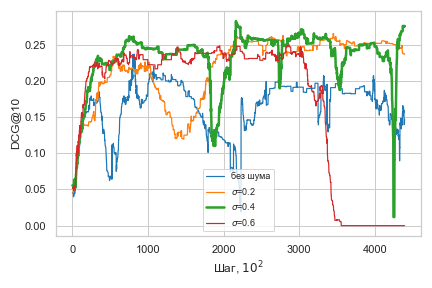
\includegraphics[scale=0.55]{img/curve_dcg.png}
	\caption{Кривая обучения DCG@10 для одного пользователя}
	\label{fig:hit_curve}
	\end{minipage}
	\hfill
	\begin{minipage}[b]{0.49\textwidth}
		\centering
		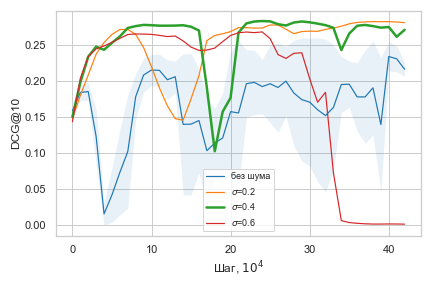
\includegraphics[scale=0.55]{img/curve_dcg_all_.png}
	\caption{Кривая обучения DCG@10 для всех пользователей}
	\label{fig:hit_curve}
		
	\end{minipage}
\end{figure}

Синим затемнением на графике отмечено стандартное отклонение по трём запускам модели без шума.

\begin{figure}[H]
	\begin{minipage}[b]{0.49\textwidth}
		\centering
		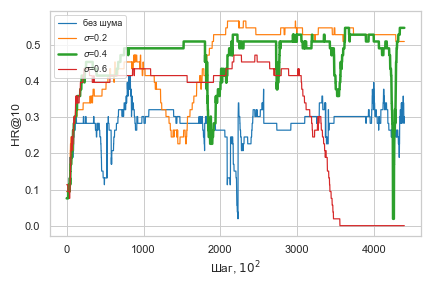
\includegraphics[scale=0.55]{img/curve_hit.png}
	\caption{Кривая обучения HR@10 для одного пользователя}  
	\label{fig:hit_curve}
	\end{minipage}
	\hfill
	\begin{minipage}[b]{0.49\textwidth}
		\centering
		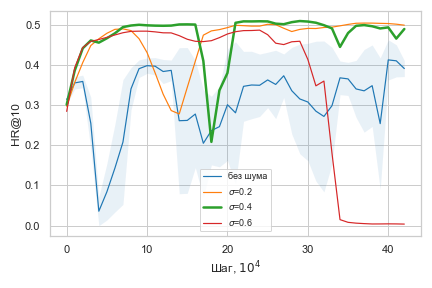
\includegraphics[scale=0.55]{img/curve_hit_all_.png}
	\caption{Кривая обучения HR@10 для всех пользователей}
	\label{fig:hit_curve}
	\end{minipage}
\end{figure}


Для итогового вычисления качества модели использовались наилучшие веса из истории оценивания по всем пользователям. Результаты представлены в таблице \ref{Tab:results}

\begin{center}
	\begin{table}[h]
		\centering
		%\begin{tabular}{l|l|l|l}
		\begin{tabular}{ccc}
			\hline Модель & DCG@10 &  HR@10 \\
			\hline $\sigma = 0.6$ & 0.268  & 0.487\\
			$\pmb{\sigma = 0.4}$  & {\bf 0.282} & {\bf 0.509} \\
			$\sigma$ = 0.2 & {\bf 0.282}  & 0.504\\
		    без шума & 0.254 & 0.454 \\
			Случайные рекомендации & $\sim 0.05$ & $\sim 0.1$   \\
			\hline 
		\end{tabular}
		\caption{Сравнение разных вариантов шума}
		\label{Tab:results}
	\end{table}
\end{center}

Видно, что использование шума повышает как итоговые критерии качества, так и их промежуточные значения в процессе обучения.

\newpage

\section{Заключение}

\subsection{Итоги работы}

В рамках проведенного исследования была достигнута поставленная цель и решены
сформулированные в начале исследования задачи. На защиту выносятся следующие результаты:
\begin{enumerate}
\item Разработана модель ранжирования рекомендаций на основе алгоритма обучения с подкреплением актор-критик с использованием стохастических процессов Орнштейна~---~Уленбека
\item Показано, что оптимизация дисперсии процессов Орнштейна~---~Уленбека улучшает качество рекомендаций по~критериям DCG и HR.
\item Показано, что детерминированные предсказания затрудняют исследование среды агентом.
\end{enumerate}

\subsection{Дальнейшие исследования}

Рассматриваются следующие возможные варианты развития данной работы:

\begin{enumerate}
\item Изучить подходы к построению состояний среды.

\item Сравнить рассмотренный в данной работе метод с другими упомянутыми перспективными алгоритмами, такими как trulyPPO \cite{trulyPPO}.
\item Исследовать более сложные постановки задач рекомендательного моделирования, включая многошаговые рекомендательные сценарии, где на каждой итерации происходит переформулировка или уточнение запроса. Такая постановка задачи близка к разведочному поиску. Обычно разведочный поиск включает в себя несколько итераций поисковых запросов, а также используется в случаях, когда пользователь не имеет четкого запроса или представления о требуемом результате поиска. Цель такого поиска — не только найти информацию, точно соответствующую запросу, но и осознать, изучить новую тему. Обучение с подкреплением --- подходящий метод для решения такой задачи. Таким образом, данное исследование может быть продолжено не только в рамках рекомендательного моделирования, но и в рамках алгоритмов поиска текстовых документов.

\end{enumerate}

Также в дальнейшем планируется перейти на использование фреймворка Catalyst (включен в Pytorch Ecosystem) \cite{catalyst}.

\newpage


%%%%%%%%%%%%%%%%%%%%%%%%%%%%%%%%%%%%%%%%%%%%%%%%%%%%%%%%%%%%%%%%%%%%%%%%%
\newpage
\addcontentsline{toc}{section}{\protect\numberline{}Список литературы}
\bibliographystyle{ugost2008}
\bibliography{recsys_rl}
\nocite{*}

\end{document} 